% 4e de couverture
\textbf{Image processing tutorials with python}
This book is a collection of tutorials and exercises given at MINES Saint-Etienne as part of the Master’s Degree in Science and Executive Engineering ("Ingénieur Civil des Mines -- ICM"). In recent years, project-based learning has been used to illustrate theoretical concepts with real and concrete applications.

Whether you are in the early years of your university studies, in preparatory classes for the French Grandes Ecoles or in an engineering school, or even as a teacher, this book is made for you. You will find a large number of tutorials, classified by field, to familiarize yourself with the theoretical concepts of image processing and analysis. 

Go to http://iptutorials.science to download the complete codes in python.

\textbf{Yann GAVET} He graduated from Mines Saint-Etienne with a Master’s Degree in Science and Executive Engineering ("Ingénieur Civil des Mines - ICM") in 2001, obtained a Master of Science in 2004 and defended his PhD thesis in 2008. He teaches signal-processing, image-processing and pattern-recognition as well as C programming at Master’s level.

\textbf{Johan DEBAYLE} He received his master of science and PhD thesis in 2002 and 2005. He is the head of the master MISPA of MINES Saint-\'Etienne, and teaches signal-processing, image-processing and pattern-recognition at Master's level.

\begin{center}
 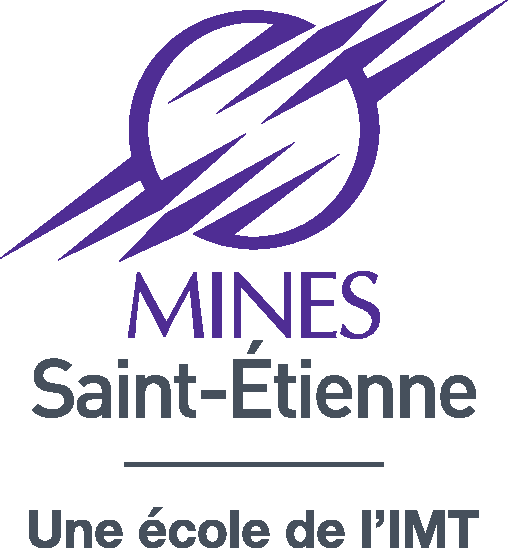
\includegraphics[width=3cm]{emse.pdf}
\end{center}
